\documentclass[
  bibliography=totoc,     % Literatur im Inhaltsverzeichnis
  captions=tableheading,  % Tabellenüberschriften
  titlepage=firstiscover, % Titelseite ist Deckblatt
]{scrartcl}

% Paket float verbessern
\usepackage{scrhack}

% Warnung, falls nochmal kompiliert werden muss
\usepackage[aux]{rerunfilecheck}

% unverzichtbare Mathe-Befehle
\usepackage{amsmath}
% viele Mathe-Symbole
\usepackage{amssymb}
% Erweiterungen für amsmath
\usepackage{mathtools}

% Fonteinstellungen
\usepackage{fontspec}
% Latin Modern Fonts werden automatisch geladen
% Alternativ:
%\setromanfont{Libertinus Serif}
%\setsansfont{Libertinus Sans}
%\setmonofont{Libertinus Mono}
\recalctypearea % Wenn man andere Schriftarten gesetzt hat,
% sollte man das Seiten-Layout neu berechnen lassen

% deutsche Spracheinstellungen
\usepackage{polyglossia}
\setmainlanguage{german}


\usepackage[
  math-style=ISO,    % ┐
  bold-style=ISO,    % │
  sans-style=italic, % │ ISO-Standard folgen
  nabla=upright,     % │
  partial=upright,   % ┘
  warnings-off={           % ┐
    mathtools-colon,       % │ unnötige Warnungen ausschalten
    mathtools-overbracket, % │
},                       % ┘
]{unicode-math}

% traditionelle Fonts für Mathematik
\setmathfont{Latin Modern Math}
% Alternativ:
%\setmathfont{Libertinus Math}

\setmathfont{XITS Math}[range={scr, bfscr}]
\setmathfont{XITS Math}[range={cal, bfcal}, StylisticSet=1]

% Zahlen und Einheiten
\usepackage[
locale=DE,                   % deutsche Einstellungen
separate-uncertainty=true,   % immer Fehler mit \pm
per-mode=symbol-or-fraction, % / in inline math, fraction in display math
]{siunitx}

% chemische Formeln
\usepackage[
version=4,
math-greek=default, % ┐ mit unicode-math zusammenarbeiten
text-greek=default, % ┘
]{mhchem}

% richtige Anführungszeichen
\usepackage[autostyle]{csquotes}

% schöne Brüche im Text
\usepackage{xfrac}

% Standardplatzierung für Floats einstellen
\usepackage{float}
\floatplacement{figure}{htbp}
\floatplacement{table}{htbp}

% Floats innerhalb einer Section halten
\usepackage[
section, % Floats innerhalb der Section halten
below,   % unterhalb der Section aber auf der selben Seite ist ok
]{placeins}

% Seite drehen für breite Tabellen: landscape Umgebung
\usepackage{pdflscape}

% Captions schöner machen.
\usepackage[
  labelfont=bf,        % Tabelle x: Abbildung y: ist jetzt fett
  font=small,          % Schrift etwas kleiner als Dokument
  width=0.9\textwidth, % maximale Breite einer Caption schmaler
]{caption}
% subfigure, subtable, subref
\usepackage{subcaption}

% Grafiken können eingebunden werden
\usepackage{graphicx}
% größere Variation von Dateinamen möglich
\usepackage{grffile}

% schöne Tabellen
\usepackage{booktabs}

% Verbesserungen am Schriftbild
\usepackage{microtype}

% Literaturverzeichnis
\usepackage[style=alphabetic,]{biblatex}
% Quellendatenbank
\addbibresource{lit.bib}

% Hyperlinks im Dokument
\usepackage[
  unicode,        % Unicode in PDF-Attributen erlauben
  pdfusetitle,    % Titel, Autoren und Datum als PDF-Attribute
  pdfcreator={},  % ┐ PDF-Attribute säubern
  pdfproducer={}, % ┘
]{hyperref}
% erweiterte Bookmarks im PDF
\usepackage{bookmark}

% Trennung von Wörtern mit Strichen
\usepackage[shortcuts]{extdash}

\title{V406: Beugung am Spalt}
\author{
  Simon Schulte
  \texorpdfstring{
    \\
    \href{mailto:simon.schulte@udo.edu}{simon.schulte@udo.edu}
  }{}
  \texorpdfstring{\and}{, }
  Tim Sedlaczek
  \texorpdfstring{
    \\
    \href{mailto:tim.sedlaczek@udo.edu}{tim.sedlaczek@udo.edu}
  }{}
}
\publishers{TU Dortmund – Fakultät Physik}

\date{Durchführung: 09.05.2017\\
      Abgabe: 16.05.2017}


\begin{document}

\maketitle
\thispagestyle{empty}
\tableofcontents
\newpage
\setcounter{page}{1}
\section{Zielsetzung}
\label{sec:zielsetzung}
Ziel des Versuchs ist die Untersuchung von Lichtbeugung an einem Einzelspalt und zwei Doppelspalten.
\section{Theorie}
\label{sec:theorie}
Die Beugung des Lichts beschreibt die Abweichung der Lichtausbreitung von den
Gesetzen der geometrischen Optik. Nach dem Huygensschen Prinzip und dem Interferenzprinzip von Fresnel werden von jedem Punkt einer Wellenfläche Elementarwellen ausgesendet. Diese breiten sich kugelwellenartig aus. Dabei interferieren sie miteinander.
\begin{figure}[htb]
  \centering
  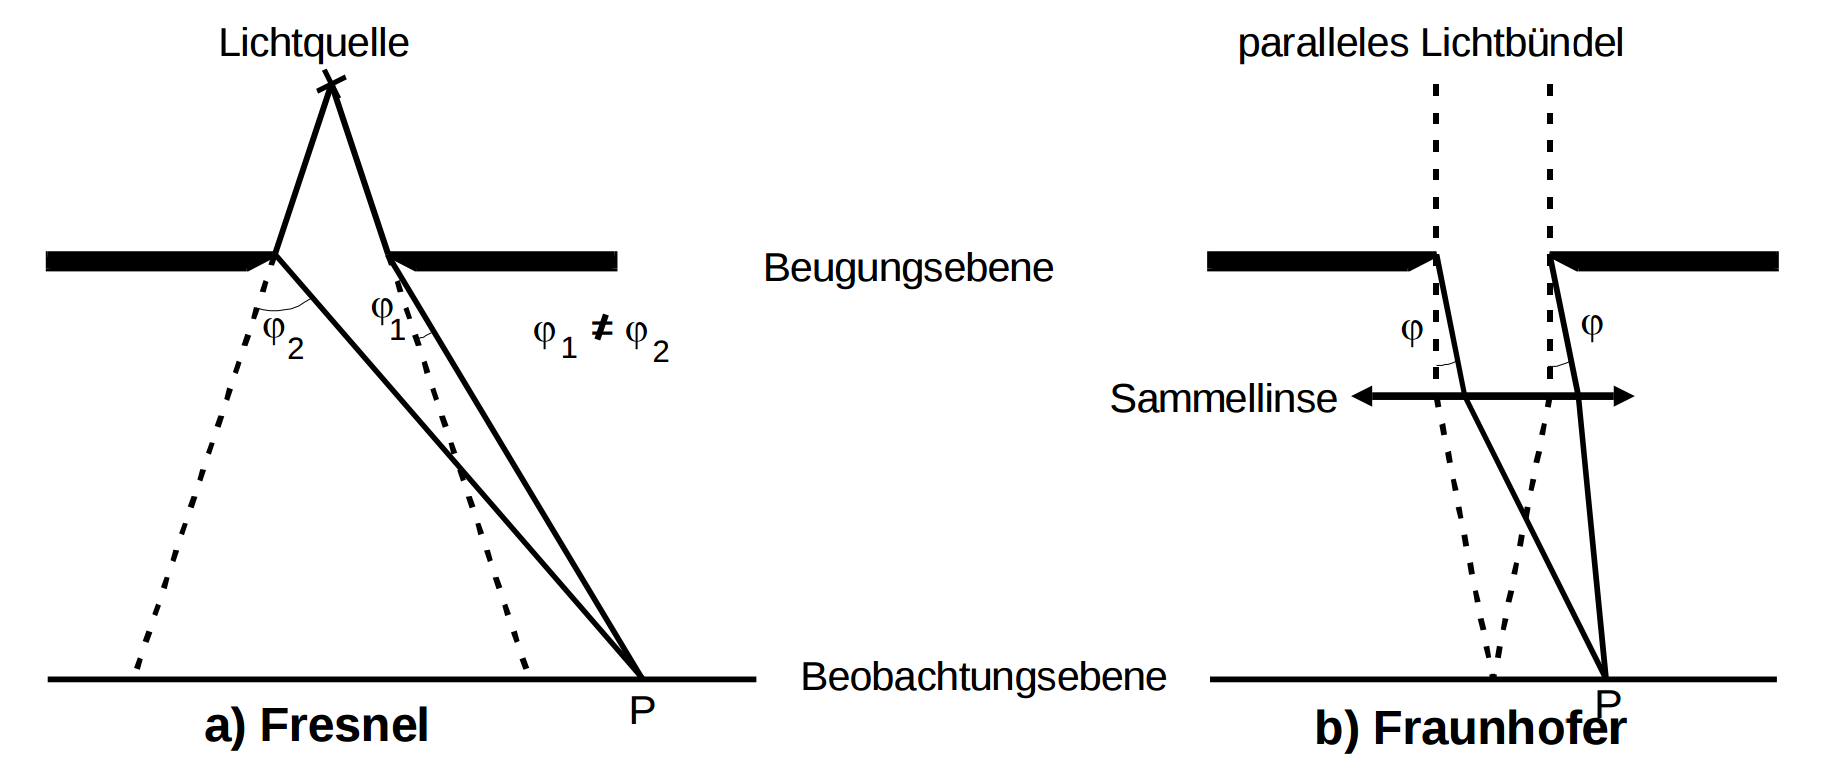
\includegraphics[width=0.9\textwidth]{V4061.png}
  \caption{Die Fesnelsche und Franhofersche Beugung an einem Einfachspalt. \cite{anleitung}}
  \label{fig:V4061}
\end{figure}
Abbildung \ref{fig:V4061} zeigt die Fresnelsche und Fraunhofersche Beugung an einem Einzelspalt. In diesem Versuch wird lediglich die Fraunhofersche Beugung betrachtet, da man diese mathematisch einfacher beschreiben kann. Hierbei wird von einem parallel ankommenden Strahl ausgegangen. Die getrichelten Linien stellen den Verlauf der geometrischen Optik dar. Bei der Fraunhoferschen Beugung werden die Lichtstrahlen aber teilweise um den Winkel $\phi$ gebeugt. Dadurch interferieren sie im Punkt $P$. Dieser Effekt hängt mit dem Huygensschen Prinzip und dem Interferenzprinzip von Fresnel zusammen. Um nun die Amplitude eines Einzelspalts zu bestimmen, muss über alle Strahlenbündel, welche um den Winkel $\phi$ ausgelenkt werden, summiert werden. Eine hier betrachtete Welle wird durch
\begin{equation}
  A(z,t)\,=\,A_0\exp\Big(i\Big(\omega t-2\pi \frac{z}{\lambda}\Big)\Big)
  \label{eqn:welle}
\end{equation}
beschrieben. Diese hat den Phasenunterschied:
\begin{equation}
  \delta\,=\,\frac{2\pi x\sin(\phi)}{\lambda}.
  \label{eqn:phasenunterschied}
\end{equation}
In Abbildung \ref{fig:V4065} wird genau dies skizziert.
\begin{figure}[htb]
  \centering
  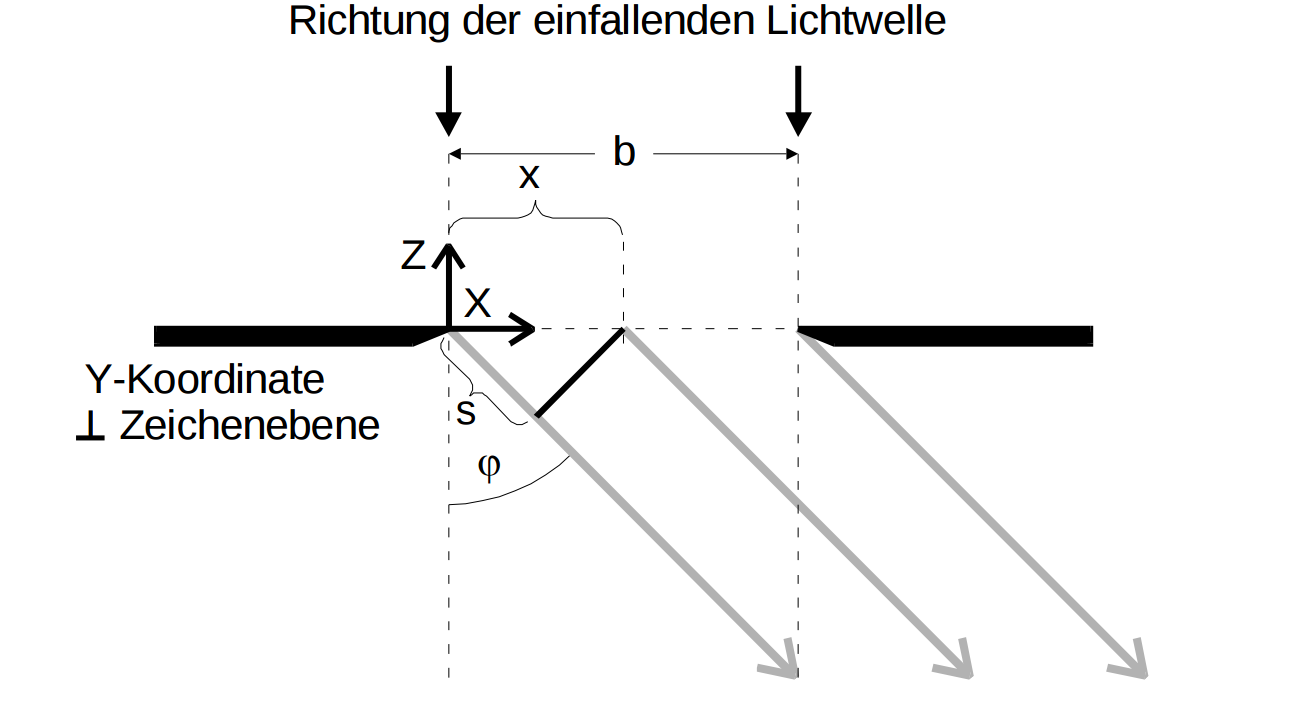
\includegraphics[width=0.9\textwidth]{V4065.png}
  \caption{Eine Skizze zur Ableitung einer Phasenbeziehung zwischen 2 Teilstrahlen bei der Fraunhoferschen Beugung am Spalt. \cite{anleitung}}
  \label{fig:V4065}
\end{figure}
Die Strahlenbündel vom Laser sind sehr klein. Daher integriert man über die Spaltbreite $D$. Dadurch ergibt sich
\begin{equation}
  B(z,t,\phi)\,=\,A_0\exp\Big(i\Big(\omega t-\frac{2\pi z}\lambda\Big)\Big)\cdot \exp\Big(\frac{\pi ib \sin(\phi)}{\lambda}\Big)\cdot\frac{\lambda}{\pi \sin(\phi)}\sin\Big(\frac{\pi b\sin{\phi}}{\lambda}\Big)
  \label{eqn:amplitude}
\end{equation}
für die Amplitude vom den in $\phi$-Richtung abgelenkten Strahlen. Da sich die Amplitude nicht direkt messen lässt, wird zur Überprüfung ebenfalls die zeitlich gemittelte Intensität $I(\phi)$ bestimmt. Dabei ergibt sich folgender Zusammenhang:
\begin{equation}
  I(\phi)\,\propto\,B(\phi)²\,=\,A_0 b²\Big(\frac{\lambda}{\pi b\sin(\phi)}\Big)²\cdot \sin²\Big(\frac{\pi b\sin(\phi)}{\lambda}\Big).
  \label{eqn:intensitätsverteilungeinzel}
\end{equation}
Ein Doppelspalt kann physikalisch auch als Überlagerung zweier Einzelspalte gesehen werden. Abbildung \ref{fig:V4064} zeigt eine Beugung am Doppelspalt, an der dies gut erkennbar ist. Dann ergibt sich für die Intensitätsverteilung eines Doppelspalts
\begin{equation}
  I(\phi)\,\propto\,B(\phi)²\,=\,4\cos²\Big(\frac{\pi s\sin(\phi)}{\lambda}\Big)\cdot\Big(\frac{\lambda}{\pi b\sin(\phi)}\Big)²\cdot \sin²\Big(\frac{\pi b\sin(\phi)}{\lambda}\Big).
  \label{eqn:intensitätsverteilungdoppel}
\end{equation}
\begin{figure}[htb]
  \centering
  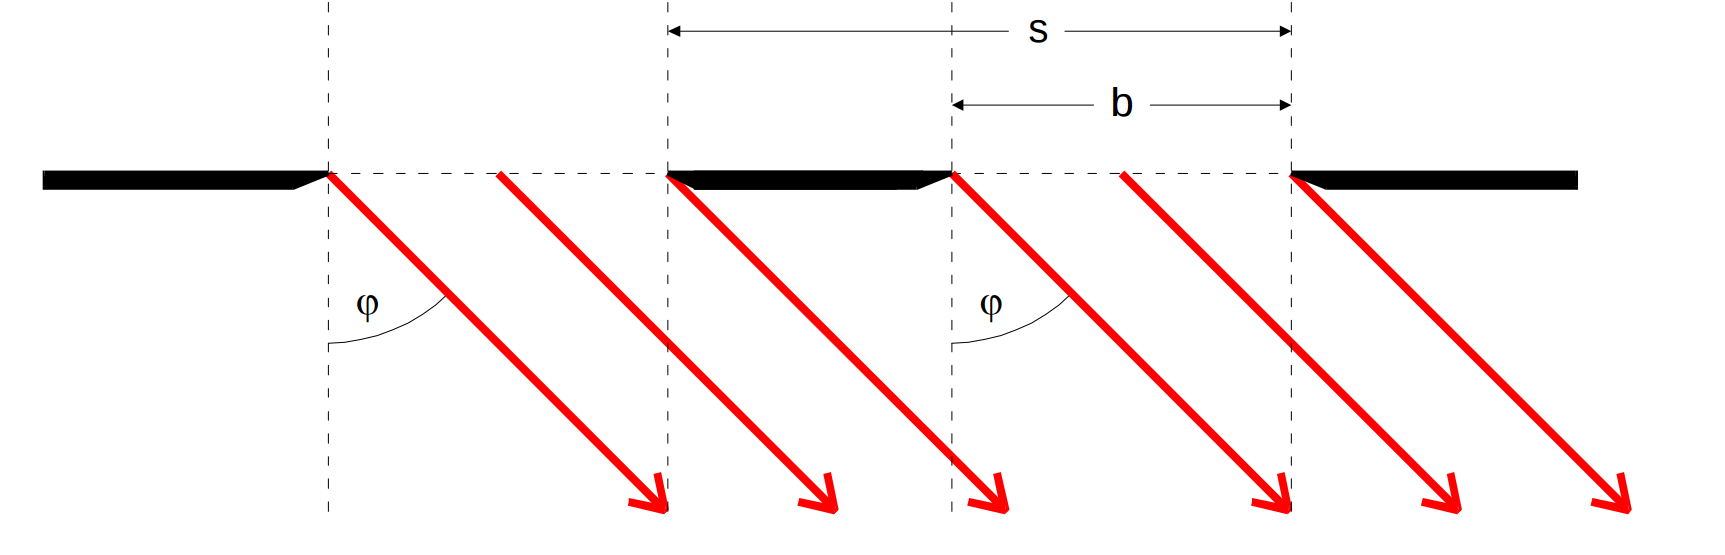
\includegraphics[width=0.9\textwidth]{V4064.png}
  \caption{Die Beugung am Doppelspalt. \cite{anleitung}}
  \label{fig:V4064}
\end{figure}

\section{Durchführung}
\subsection{Versuchsaufbau}
\label{sec:Versuchsaufbau}
\begin{figure}[htb]
  \centering
  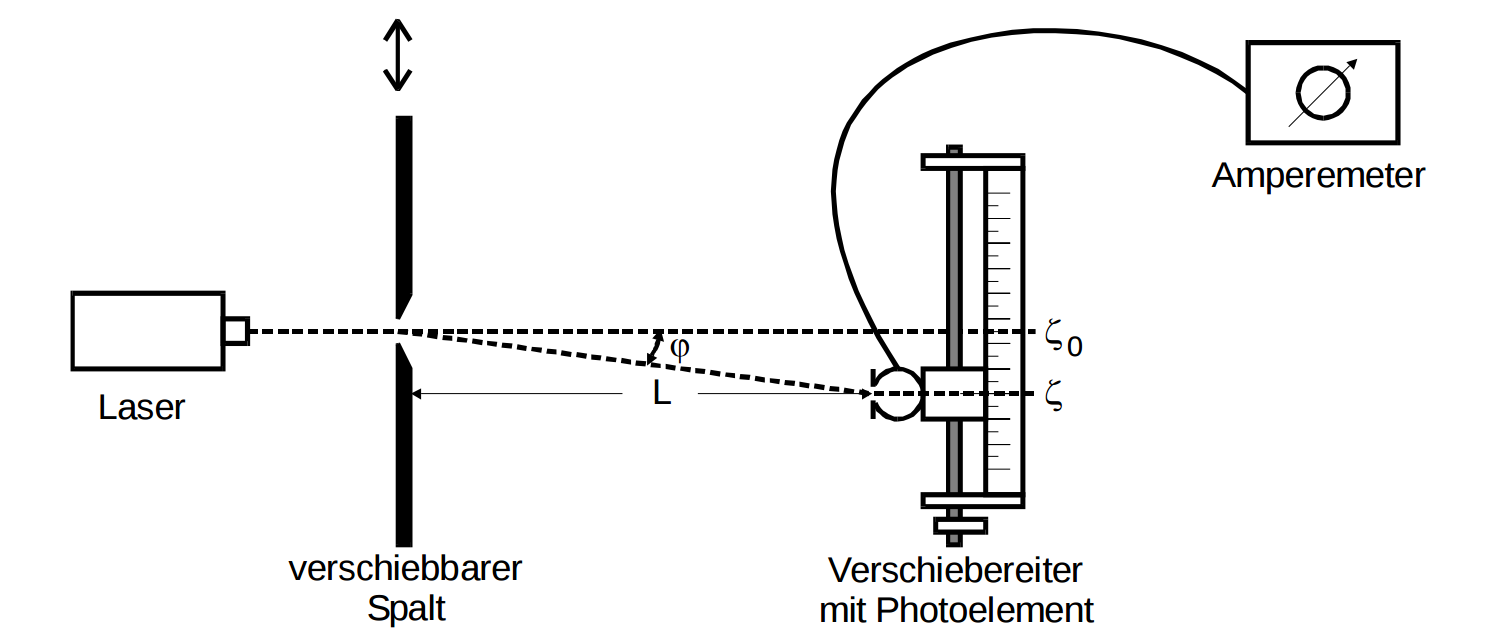
\includegraphics[width=0.9\textwidth]{V4063.png}
  \caption{Der Versuchsaufbau zur Ausmessung einer Beugungsfigur. \cite{anleitung}}
  \label{fig:V4063}
\end{figure}
In Abbildung \ref{fig:V4063} zu sehen ist der in dem Versuch verwendete Versuchsaufbau. Ein Laser sendet Lichtwellen mit einer Wellenlänge von \SI{635}{\nano\metre} aus. Dies ist notwendig, da Lichtbeugung nur auftritt, wenn der Spalt, an dem es gebeugt wird, ungefähr der Größenordnung der Wellenlänge $\lambda$ entspricht. Die Lichtwellen gehen durch einen Spalt, welcher in dem Versuch drei mal variiert wird. Dann kommen die Lichtwellen nach einer Strecke von L=\SI{124}{\centi\metre} an einem Verschiebereiter mit Photoelement an. Dieser misst die Intensität der einlaufenden Welle und schickt die Information an ein Amperemeter, an welchem man dann den Diodenstrom ablesen kann.
\subsection{Versuchsablauf}
\label{sec:Versuchsablauf}
Als erstes werden die Spaltbreiten $D$ und die Gitterkonstanten $g$ des jeweiligen verwendeten Spaltes bestimmt.
Die ergeben sich für den Einfachspalt zu
\begin{align}
  D_{Einfachspalt}\,=\,\SI{0.075}{\milli\metre}
  \label{eqn:einfachspalt}
\end{align}
Für den ersten verwendeten Doppelspalt ergibt sich
\begin{align}
  D_{Doppelspalt 1}\,=\,\SI{0.1}{\milli\metre}\\
  g_{Doppelspalt 1}\,=\,\SI{0.4}{\milli\metre}.
  \label{eqn:doppelspalt1}
\end{align}
Für den zweiten verwendeten Doppelspalt ergibt sich
\begin{align}
  D_{Doppelspalt 2}\,=\,\SI{0.15}{\milli\metre}\\
  g_{Doppelspalt 2}\,=\,\SI{0.25}{\milli\metre}.
  \label{eqn:doppelspalt2}
\end{align}
Danach misst man, was für einen Diodenstrom das Amperemeter registriert, wenn der Laser noch nicht eingeschaltet ist. Dies nennt man Dunkelmessung und dieser Wert wird dann von den anderen Werten abgezogen, da die Lichtwellen, die sich im Raum befinden und auf das Amperemeter treffen die Messung verfälschen. Die Dunkelmessung ergab einen Wert von
\begin{equation}
  A_{Dunkel}\,=\,\SI{1.15}{\nano\ampere}.
  \label{eqn:dunkel}
\end{equation}
Danach werden 93 Werte im Bereich von \SI{1}{\milli\metre} bis \SI{50}{\milli\metre} am Verschiebereiter mit Photoelement für den Diodenstrom aufgenommen. Dazu wird ein Einfachspalt verwendet.
Als nächstes werden 56 Werte zwischen \SI{14.25}{\milli\metre} und \SI{40.25}{\milli\metre} für den Diodenstrom aufgenommen. Dazu wird der erste Doppelspalt verwendet.
Als letztes werden 50 Werte im Bereich von \SI{11.25}{\milli\metre} bis \SI{40.75}{\milli\metre} für den Diodenstrom aufgenommen. Dazu wird der zweite Doppelspalt verwendet.
\end{document}
